\documentclass[11pt,a4paper]{article}
\title{APG4011F Bundle Adjustment Report}
\date{21 April 2015}
\author{Tim Marsh}

\usepackage{amsmath}
\usepackage{graphicx}
\usepackage{float}
\usepackage{textcomp}
\usepackage{siunitx}
\usepackage{wrapfig}
\usepackage{caption}
\usepackage{subcaption}

\usepackage[margin=1in]{geometry}

\graphicspath{ {./} }
\begin{document}
	
	\pagenumbering{gobble}
	\maketitle
	\begin{figure}[H]
		\centering
		
\includegraphics[width=0.7\linewidth]{images/UCTcircular_logo1_CMYK}
		\label{fig:UCTcircular_logo1_CMYK}
	\end{figure}
	\newpage
	\pagenumbering{arabic}
	\tableofcontents
	\listoffigures
	\newpage
	
	
	\section{Introduction}
	
	There are three parts to this assignment:
	
	\begin{description}
			\item[1. Simulating a camera, image points and object points] Creating the Cameras with made up parameters, $Xo$, $Yo$, $Zo$, $\kappa$, $\phi$, $\omega$. Creating 30 image points and calculating the corresponding ground coordinates for those image points.
			
			\item[2. Intersection] After creating a new camera, with its own orientation parameters, calculate the corresponding image point coordinates.
			
			Then using least squares calculate the best fit ground coordinates for both images.
			
			\item[3. Resection] Using the object coordinates from part 1 along with the corresponding image points, set up a least squares solution solution to determine the exterior orientation parameters of the image. do this for both images
			
			\item[4. Bundle adjustment] Treat 25 of the 30 points as control points and the remaining 5 as tie points. Use the collinearity equations to setup a least squares solution to simultaneously determine the exterior orientation parameters of the two images and the object coordinates of the tie points.
			
	\end{description}
	
	These 4 parts are done as one single program written in python that runs from start to finish. the first two cameras are defined with orientation parameters, object points and image points. Each time some action needs to be preformed on a camera a new camera instance is created and the things that need to be calculated are cleared, calculated and saved in the new instance so that they can be compared to the original values.
	
	\section{Program structure}
	
	im order to store a lot of information in a program without losing any, and being able to access it whenever is necessary. This is done with dictionaries within dictionaries.
	
	The main dictionary is Cameras, Cameras holds the image size as well as the focal length of the camera (the focal length is constant through all images). in the Cameras dictionary are Images there are multiple images (in this case 2) the Images class holds the exterior orientation parameters of that Image(photograph).
	
	Each image has image points and object points, to keep the image points and object points paired up in created and saved them in a ray class. It holds no information other than keeping the image and object points paired up.
	
	Figure 1 shows a very basic representation of the structure.
	
	\begin{figure}[H]
		\centering
		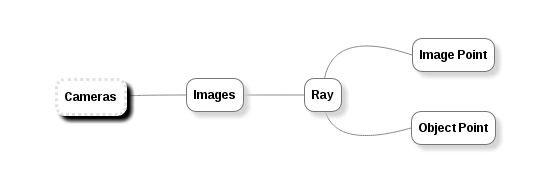
\includegraphics[width=0.7\linewidth]{/images/crop}
		\caption{Structure of Dictionaries}
		\label{fig:structure}
	\end{figure}


	\section{Background to the Problem}
	
	Knowledge of how photogrammetry works is necessary for this assignment. Each image has its image center $Xo$ $Yo$ $Zo$ as well as rotations around the $x$ $y$ and $z$ axes, $\kappa$ $\phi$ $\omega$. 
	
	\section{Method}
	
	In the first part ground coordinates are calculated using the collinearity equations. the basic form of the collinearity equations take object points or image points and calculates the other.\\
	\\
	
	
	\centerline{
	$
	\begin{bmatrix}
		X - Xo \\ 
		Y - Yo \\ 
		Z - Zo
	\end{bmatrix}= kR^T$
	$
	\begin{bmatrix}
		y \\ 
		x \\ 
		-c
	\end{bmatrix}
	$
	where R = $R\kappa R\phi R\omega$ and $k$ = scale\\}
	~\\
	
	In the second part this formula is reversed so that image coordinates are being calculated from the object points calculated in part 1.
	
	These are easy steps and involve going through each point in the images and calculating its corresponding point in either the image or object space. Part 3 and 4 are more complex and involve least squares to solve.\\
	
	Part 3 consists of calculating the exterior orientation parameters for an image having only image and object points. this is done through least squares. 
	
	There are 6 unknowns; $Xo$, $Yo$, $Zo$, $\kappa$, $\phi$, $\omega$ as well as a scale ($s_i$) for each point (You can see the new scale being brought in inn the last term of each equation below). This means that for every point you add in one more unknown must be added. Each point brings 3 equations:
	
	\begin{equation}\notag
	U_i - \tilde{X_i} = \tilde{Y_i} dk + \tilde{Z_i}d\phi + X_o + \tilde{X_i}ds_i
	\end{equation}
	\begin{equation}\notag
	V_i - \tilde{Y_i} = \tilde{Y_i} dk - \tilde{Z_i}d\omega + Y_o + \tilde{Y_i}ds_i
	\end{equation}
	\begin{equation}\notag
	W_i - \tilde{Z_i} = -\tilde{Y_i} dk + \tilde{Y_i}d\omega + Z_o + \tilde{Z_i}ds_i
	\end{equation}
	
	There needs to be a minimum of 9 equations to solve the 6 unknowns as well as the scale being brought in. This is no problem for us because we have 30 points, which are more than enough to solve this.
	
	From here we solve the seytem of equations using least squares as we would normal. create the $A$ matrix and $\ell$ matrix then solve for $X$.
	\begin{equation}
	X = (A^T A)^{-1} A^T\ell
	\end{equation}
	The $X$ matrix will be our 6 unknowns followed by a scale for each point.\\
	
	Part 4 is what we call relative orientation, we are taking 2 camera with unknown $Xo$, $Yo$, $Zo$, $\kappa$, $\phi$, $\omega$ and orientating them relative to each other to create a stereo-model. So you would expect there to be 12 unknowns along with the point scales. But this is not solvable because there are to many unknowns. But this is still a solvable problem.
	We do not need all 12 variables to relativity orientate the 2 images. we only need 5. 5 Rotations or 2 translations and 3 rotations. once the two images are relatively orientated we must transfer them into the object coordinates.
	
	This problem is once again solved using least squares.
	
	
	\section{Results}
	
	The results of this are hard to showcase with out some graphical representation. Starting off with a single camera and its image points then creating its object points results in a situation as shown in Figure 2 below. Figure 2 shows 30 points from a single camera as calculated in part 1. This image was generated using the code after part 1. 
	
	\begin{figure}[H]
		\centering
		\includegraphics[width=0.7\linewidth]{"/images/one30"}
		\caption{Single Camera View}
		\label{fig:oneimage}
	\end{figure}
	
	After part 2 and 3 a second camera had been created and displayed as in Figure 3.
		
	\begin{figure}[H]
		\centering
		\includegraphics[width=0.7\linewidth]{"/images/two30"}
		\caption{Two Cameras View }
		\label{fig:twoimages}
	\end{figure}
	
	After part 4 the image produces was very much the same as in Figure 3.
	
\end{document}	